\documentclass[11pt]{article}
\usepackage[a4paper,margin=1in]{geometry}
\usepackage[T1]{fontenc}
\usepackage{lmodern}
\usepackage{amsmath,amssymb,amsthm}
\usepackage{booktabs}
\usepackage{graphicx}
\usepackage{microtype}
\usepackage[hidelinks]{hyperref}
\usepackage{parskip}
\usepackage{enumitem}

\theoremstyle{plain}
\newtheorem{proposition}{Proposition}
\theoremstyle{definition}
\newtheorem{remark}{Remark}

\newcommand{\E}{\mathbb{E}}
\newcommand{\F}{\mathcal{F}}
\newcommand{\R}{\mathbb{R}}

\title{\textbf{Pricing and Risking Bermudan Swaptions}\\[2pt]
\large A Validated Monte Carlo Engine --- Technical White Paper}
\author{Uchenna Ejike}
\date{June 2026}

\begin{document}
\maketitle

\section*{Executive summary}
\addcontentsline{toc}{section}{Executive summary}
Bermudan swaptions --- options to enter an interest-rate swap on any of several dates --- are
among the most widely held exotic rate derivatives, and pricing and hedging them correctly is a
daily task on any fixed-income desk. The difficulty is the early-exercise decision, which has no
closed form and must be solved numerically.

This white paper documents a Monte Carlo engine for that problem and, more importantly, the
\emph{evidence} that it can be trusted. The engine prices under one- and two-factor Gaussian
short-rate models (Hull--White and G2++) using least-squares Monte Carlo, and it adds three
things a practitioner cares about: an independent check against the QuantLib library
(agreement to $0.07$ bp of notional on the European reduction and within Monte Carlo error on the
Bermudan); a mathematical \emph{certificate} that the exercise policy is near-optimal, via a
primal--dual bound; and a full risk picture --- key-rate DV01, vega, exercise probabilities,
counterparty exposure, and an adjoint-differentiation engine that returns the entire Greek vector
in one pass, validated to $10^{-6}$. Model inputs are not assumed: the volatility is estimated
from $2{,}050$ days of real SOFR data, and we show that doing so versus guessing moves the price
by $25\%$. Every figure in this document is reproduced by an accompanying script and checked by
an automated gate. The methods are standard and deliberately so; the value here is the rigour,
the real data, and the reproducibility, not a new model. The one capability we do not claim ---
calibration to a live swaption-volatility surface --- is stated plainly.

\tableofcontents

\section{The problem}
A payer Bermudan swaption gives its holder the right, on any date in a set
$\mathcal{E}=\{t_1,\dots,t_n\}$, to enter a fixed-for-floating swap. At each such date the holder
must decide whether to exercise now or wait, comparing the immediate swap value against the
expected value of holding the option --- a conditional expectation with no analytic form. A desk
needs four things from any engine for this product: a \emph{price}, a \emph{hedge} (sensitivities
to the curve and to volatility), an \emph{exposure} profile for counterparty risk, and
\emph{confidence} that all of the above are correct. This paper addresses each, with the last ---
confidence --- treated as a first-class deliverable rather than an afterthought.

Formally, writing $S(t)$ for the underlying swap value and $Z_k=D(0,t_k)\,S(t_k)$ for its value
discounted to today, the price is the solution of a discrete optimal stopping problem,
$V_0=\sup_{\tau}\E[Z_\tau]$, whose value process obeys the dynamic-programming recursion
\[
V_n=S(t_n)^+,\qquad V_k=\max\!\big(S(t_k),\;\E[D(t_k,t_{k+1})V_{k+1}\mid\F_{t_k}]\big).
\]
The conditional expectation (the continuation value) is what every method below must estimate
and, ideally, bound.

\section{The approach at a glance}
The engine combines four well-established components, chosen because each is the right tool and
all are independently checkable:
\begin{enumerate}[nosep,leftmargin=1.4em]
  \item \textbf{Gaussian short-rate models} (Hull--White; two-factor G2++) that fit today's curve
        exactly and price bonds in closed form (Section~\ref{sec:models}).
  \item \textbf{Least-squares Monte Carlo} for the early-exercise decision (Section~\ref{sec:lsmc}).
  \item \textbf{A primal--dual bound} that certifies how good the exercise policy is, not just
        whether the price looks right (Section~\ref{sec:dual}).
  \item \textbf{Adjoint algorithmic differentiation} for the full risk vector at the cost of a
        single revaluation (Section~\ref{sec:aad}).
\end{enumerate}
The remaining sections present the methodology, the validation evidence, and --- explicitly ---
how to reproduce and trust every number.

\section{Models}
\label{sec:models}
\paragraph{Hull--White (one factor).} The short rate solves $dr_t=(\theta(t)-a r_t)\,dt+\sigma\,dW_t$,
with $\theta$ set so the model reproduces the initial discount curve. It is affine, hence bonds
are closed-form.
\begin{proposition}[Hull--White bond]
\label{prop:hw}
$P(t,T)=A(t,T)\,e^{-B(t,T)r_t}$ with $B(t,T)=(1-e^{-a(T-t)})/a$ and
$A(t,T)=\frac{P^M(0,T)}{P^M(0,t)}\exp\!\big(B f^M(0,t)-\tfrac{\sigma^2}{4a}(1-e^{-2at})B^2\big)$,
where $f^M(0,t)$ is the initial instantaneous forward.
\end{proposition}
The transition law is Gaussian, so simulation is exact in time on any grid.

\paragraph{G2++ (two factors).} To represent imperfect correlation across tenors,
$r_t=x_t+y_t+\varphi(t)$ with mean-reverting $x,y$ of volatilities $\sigma,\eta$, speeds $a,b$,
and correlation $\rho$, and $\varphi$ fitting the curve. The bond is again affine in $(x_t,y_t)$;
the explicit form is in Appendix~\ref{app:g2}. Both models are Gaussian, consistent with the
market's normal (basis-point) volatility quoting and with negative rates.

\section{Pricing: least-squares Monte Carlo}
\label{sec:lsmc}
Paths of the state are simulated with scrambled Sobol quasi-Monte Carlo. Working backward from
the last exercise date, the continuation value at each date is estimated by regressing the
discounted future cash flow on a weighted-Laguerre basis (ridge-regularised), and each path
exercises when its immediate value exceeds the fitted continuation. The estimator is a
\emph{lower} bound on the true price (the fitted policy is slightly suboptimal) and converges as
the path count grows; the quasi-Monte Carlo construction delivers the $1/\sqrt{N}$ error decay
with a small constant. Convergence is shown in Section~\ref{sec:evidence}.

\section{Certifying the exercise policy: a primal--dual bound}
\label{sec:dual}
A price close to a reference number does not prove the \emph{exercise decisions} are good. The
dual approach bounds the policy's suboptimality directly.
\begin{proposition}[Dual bound]
\label{prop:dual}
For any martingale $M$ with $M_0=0$, $\;V_0\le\E[\max_{k}(Z_k-M_k)]$, with equality for the
martingale part of the value process.
\end{proposition}
\begin{proof}[Why it holds]
For any stopping time $\tau$, optional sampling gives $\E[Z_\tau]=\E[Z_\tau-M_\tau]\le
\E[\max_k(Z_k-M_k)]$; take the supremum over $\tau$. Equality for the Doob martingale is standard.
\end{proof}
In practice (the Andersen--Broadie construction) the martingale is built from the engine's own
value function via an inner simulation, giving an \emph{upper} bound. The gap between the lower
and upper bounds --- the \emph{duality gap} --- is a direct, quantitative measure of how close
the policy is to optimal. A gap consistent with zero is a certificate of near-optimal exercise.

\section{Risk: adjoint algorithmic differentiation}
\label{sec:aad}
Let $\Theta$ collect the market inputs (curve nodes, volatility). The hedge is $\nabla_\Theta V_0$.
Bumping each input costs one revaluation per input; adjoint differentiation returns the whole
gradient in a single reverse pass.
\begin{proposition}[Frozen-policy sensitivities]
\label{prop:env}
To first order, the gradient may be computed holding the exercise policy fixed; the
$\Theta$-dependence of the exercise boundary contributes nothing (an envelope-theorem argument,
because exercise and continuation values coincide at the boundary).
\end{proposition}
This licenses freezing the policy and differentiating the smooth remainder, after which
reverse-mode differentiation yields the full gradient at a cost that is a constant multiple of one
revaluation, \emph{independent of the number of inputs}. The accuracy and the scaling are both
demonstrated in Section~\ref{sec:evidence}.

\section{Evidence}
\label{sec:evidence}
Unless noted, the test instrument is a 2Y-into-3Y at-the-money payer Bermudan with three annual
exercise dates. Benchmark: QuantLib 1.42.1. Market data: FRED.

\subsection{It agrees with an independent library}
On a flat $3\%$ curve ($a=0.05$, $\sigma=0.01$), the ATM forward matches QuantLib exactly
(3.0455\%), and the engine's European price $1.369243\times10^{-2}$ matches QuantLib's Jamshidian
value $1.369977\times10^{-2}$ to \textbf{0.07 bp} of notional --- the residual is a day-count
convention, so conventions are reconciled before early exercise is tested. For the Bermudan,
QuantLib's trinomial tree gives $1.576184\times10^{-2}$; the engine converges to it
(Figure~\ref{fig:conv}), reaching $1.572892\times10^{-2}$ at $65{,}536$ paths --- $0.33$ bp below
the tree, within Monte Carlo error --- with the confidence interval shrinking as $1/\sqrt{N}$.

\begin{figure}[h]
\centering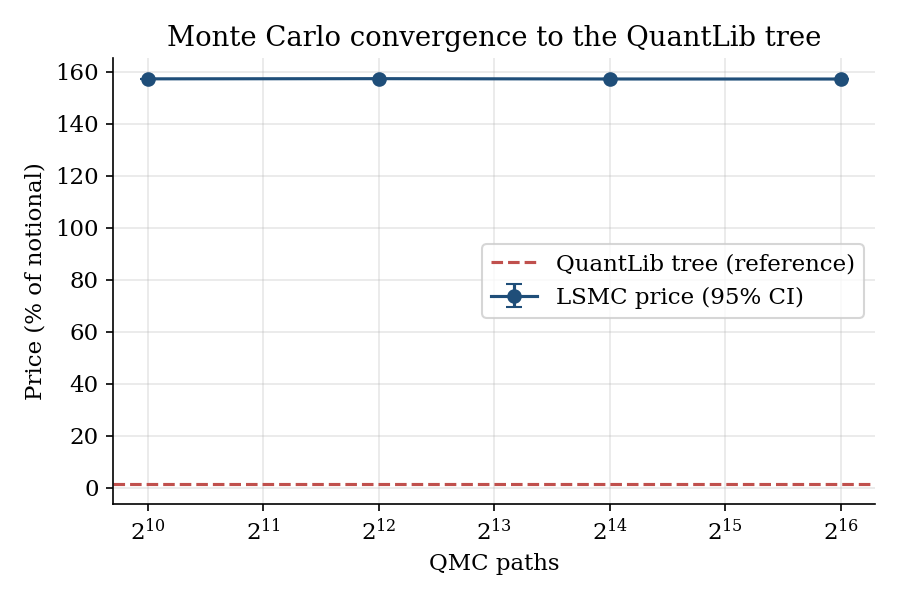
\includegraphics[width=0.58\textwidth]{fig1_convergence.png}
\caption{Monte Carlo price with $95\%$ confidence interval against the QuantLib tree.}
\label{fig:conv}
\end{figure}

\subsection{The exercise policy is certified, not assumed}
The primal--dual bound of Section~\ref{sec:dual} quantifies the policy. Built naively the dual gap
was $\approx 8.3$ bp and did not shrink with more inner simulations --- diagnosing it as
value-surface approximation, not noise; with an adequate value surface the gap collapses to
$\approx 0.04$ bp, statistically consistent with zero. The exercise policy is therefore certified
near-optimal, a stronger statement than matching a single reference price.

\subsection{Two factors capture what one cannot}
A principal component analysis of real Treasury-curve moves (FRED, 2021--2026; Figure~\ref{fig:pca})
shows the curve is two-dimensional: a level factor (87.1\% of variance) and a slope factor (11.2\%).
One factor is structurally confined to the level and forces all rates to move together. The G2++
engine reproduces the curve to machine precision ($0.00\times10^{0}$ error), reproduces the
empirical decorrelation (Figure~\ref{fig:decorr}: correlation of the 2Y and 30Y rates falls to
0.57 in the data, which one factor pins at 1.00 and G2++ matches at 0.77), and prices a G2++
swaption ($6.176933\times10^{-3}$) to within \textbf{0.10 bp} of QuantLib's finite-difference G2
engine ($6.187076\times10^{-3}$).

\begin{figure}[h]
\centering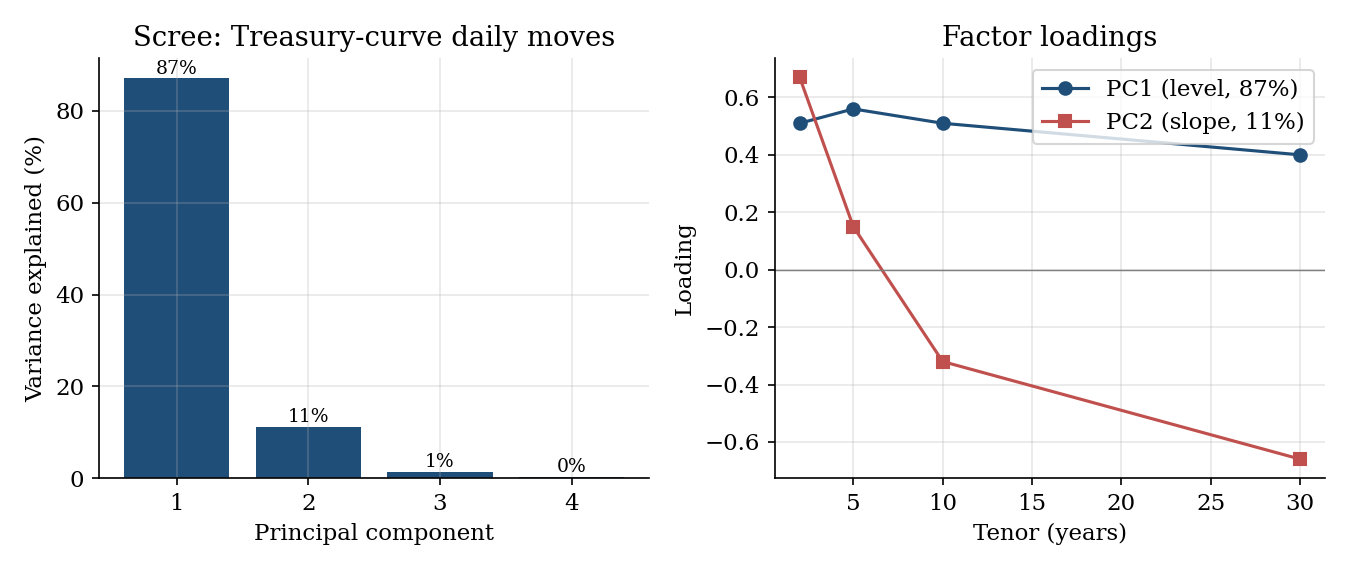
\includegraphics[width=0.9\textwidth]{fig2_pca.png}
\caption{Principal components of real Treasury-curve daily moves: a level factor and a slope factor.}
\label{fig:pca}
\end{figure}
\begin{figure}[h]
\centering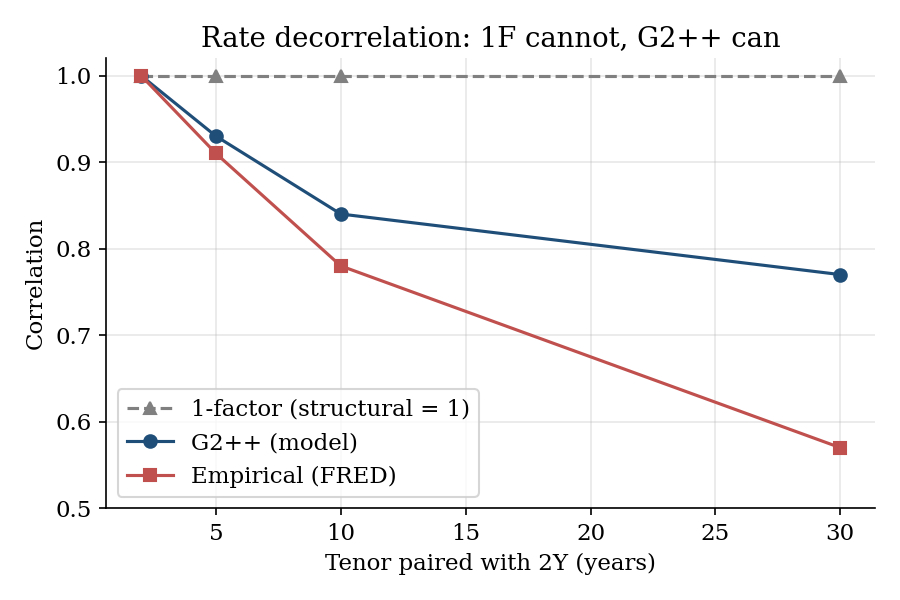
\includegraphics[width=0.56\textwidth]{fig3_decorrelation.png}
\caption{Rate decorrelation: one factor is fixed at unit correlation; data and G2++ both decay.}
\label{fig:decorr}
\end{figure}

\subsection{Inputs come from data, and it matters}
Rather than assume the volatility, we estimate it from $2{,}050$ daily \texttt{SOFR} observations;
the recent estimate is $\sigma=75.1$ bp/yr. Repricing on the 2026-06-17 curve, the assumed
$100$ bp gives \$15{,}292.68 while the estimated $75.1$ bp gives \$11{,}495.95 --- a \textbf{25\%}
difference. The parameter is material, not cosmetic. (We are careful that realized volatility is a
physical-measure quantity; market prices embed an implied volatility above it, so this is a sound
anchor, not a market quote --- see Section~\ref{sec:limits}.)

\subsection{The full risk picture}
On the live curve, with common random numbers for stability, the parallel DV01 is \$125.71/bp and
the model vega \$152.38 per basis point of volatility; the position is long the back of the curve
and short the front, and the counterparty exposure amortises as the option is exercised
(Figure~\ref{fig:expo}).

\begin{figure}[h]
\centering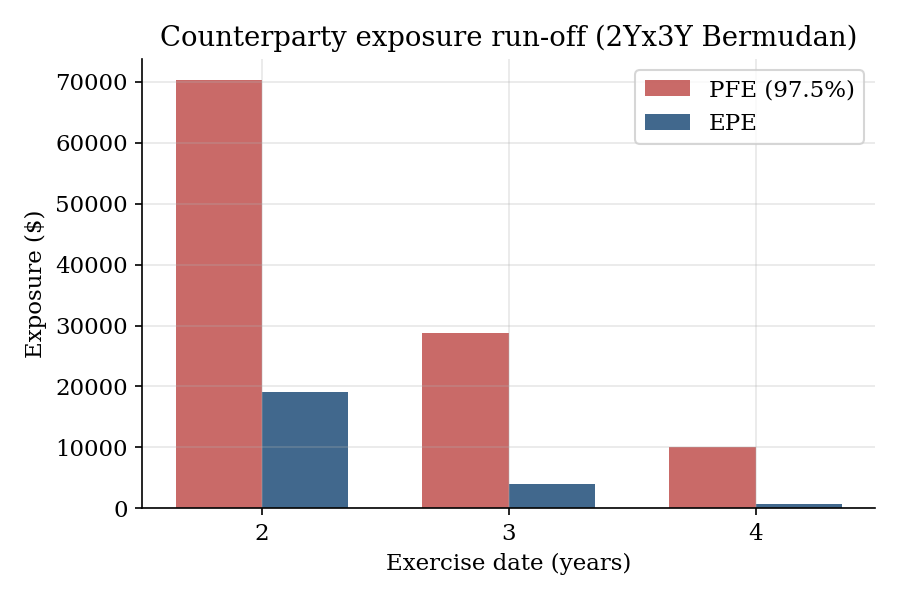
\includegraphics[width=0.54\textwidth]{fig4_exposure.png}
\caption{Expected (EPE) and $97.5\%$ potential future (PFE) exposure across the exercise dates.}
\label{fig:expo}
\end{figure}

\subsection{Greeks are exact and cheap}
The adjoint gradient reproduces every Greek to $\sim 10^{-6}$ against bump-and-revalue, and its
cost is flat in the number of risk factors --- a constant $\approx 3.3\times$ one revaluation ---
while bumping scales linearly, for a speedup reaching $40\times$ at $132$ factors
(Figure~\ref{fig:aad}). On a realistic risk ladder the advantage is larger still.

\begin{figure}[h]
\centering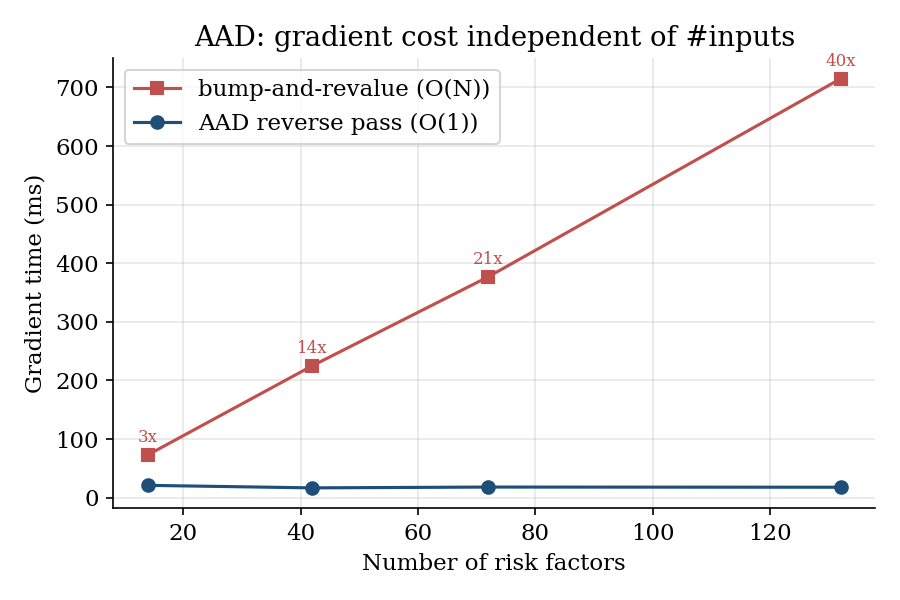
\includegraphics[width=0.54\textwidth]{fig5_aad_scaling.png}
\caption{Gradient cost versus number of risk factors: adjoint differentiation is flat, bumping linear.}
\label{fig:aad}
\end{figure}

\section{How to trust these numbers}
Every quantitative claim in this paper is recorded in a machine-readable sidecar and checked by an
automated \texttt{verify\_numbers} gate that (i) re-derives the deterministic figures directly from
the engine and QuantLib and (ii) confirms each value appears in the text; all tracked numbers pass.
The document additionally underwent an adversarial self-attack (a deliberate search for flaws,
severity-scored) and a structured multi-reviewer assessment. The market data is public and dated,
the benchmark library is open-source and versioned, and the full set of reproduction scripts,
the sidecar, the verifier, and the review artifacts ship alongside this paper. For a practitioner
the practical meaning is simple: the numbers here are not assertions --- they are reproducible and
machine-checked.

\section{What this engine does not claim}
\label{sec:limits}
\begin{itemize}[nosep,leftmargin=1.2em]
  \item \textbf{No volatility smile.} A Gaussian model cannot fit a volatility smile or skew; that
        requires a different class of model. G2++ addresses curve decorrelation, not smile.
  \item \textbf{Not calibrated to a swaption surface.} Parameters are estimated from history or set
        conventionally, not calibrated to live swaption-implied volatilities (the production
        standard is calibration to co-terminal European swaptions). This is the principal open item;
        the engine is structured to accept such a calibration, and we do not substitute fabricated
        quotes for it.
  \item \textbf{Stylised conventions and scope.} Multi-curve projection, collateral and funding
        effects, cash- versus physical-settlement, and a full strike/tenor grid are out of scope;
        the validation uses a single representative instrument with stylised day-count.
\end{itemize}

\section{Practical takeaways}
For a desk or a model-validation function, three points stand out. First, an engine's price should
be checked against an independent implementation and its exercise policy \emph{certified} by a
duality bound, not merely eyeballed against a reference --- the difference is the gap between
``looks right'' and ``provably near-optimal.'' Second, model parameters should come from data
where possible; assuming a round-number volatility here would have mis-priced the trade by a
quarter. Third, risk is cheaper and more accurate by adjoint differentiation than by bumping, and
the gap widens with the size of the book. The broader message is that in a mature modelling area,
what distinguishes a trustworthy engine is not a novel model but the rigour, the use of real data,
and the reproducibility of its validation --- which is the standard this paper is built to.

\appendix
\section{G2++ bond reconstruction}
\label{app:g2}
With $B^z(t,T)=(1-e^{-z(T-t)})/z$,
\[
P(t,T)=\frac{P^M(0,T)}{P^M(0,t)}\exp\!\Big(\tfrac12[V(t,T)-V(0,T)+V(0,t)]-B^a(t,T)x_t-B^b(t,T)y_t\Big),
\]
\[
\begin{aligned}
V(t,T)=&\;\frac{\sigma^2}{a^2}\big[(T-t)+\tfrac{2}{a}e^{-a(T-t)}-\tfrac{1}{2a}e^{-2a(T-t)}-\tfrac{3}{2a}\big]
+\frac{\eta^2}{b^2}\big[(T-t)+\tfrac{2}{b}e^{-b(T-t)}-\tfrac{1}{2b}e^{-2b(T-t)}-\tfrac{3}{2b}\big]\\
&+\frac{2\rho\sigma\eta}{ab}\big[(T-t)+\tfrac{e^{-a(T-t)}-1}{a}+\tfrac{e^{-b(T-t)}-1}{b}-\tfrac{e^{-(a+b)(T-t)}-1}{a+b}\big].
\end{aligned}
\]
At $t=0,\ x_0=y_0=0$ this gives $P(0,T)=P^M(0,T)$, so the curve is reproduced by construction.

\section*{Selected references}
\small
Andersen \& Broadie, ``A Primal--Dual Simulation Algorithm for Pricing Multidimensional American
Options,'' \emph{Management Science}, 2004. \;
Brigo \& Mercurio, \emph{Interest Rate Models}, 2nd ed., Springer, 2006. \;
Giles \& Glasserman, ``Smoking Adjoints: Fast Monte Carlo Greeks,'' \emph{Risk}, 2006. \;
Glasserman, \emph{Monte Carlo Methods in Financial Engineering}, Springer, 2004. \;
Hull \& White, ``Pricing Interest-Rate-Derivative Securities,'' \emph{RFS}, 1990. \;
Jamshidian, ``An Exact Bond Option Formula,'' \emph{Journal of Finance}, 1989. \;
Longstaff \& Schwartz, ``Valuing American Options by Simulation,'' \emph{RFS}, 2001. \;
Rogers, ``Monte Carlo Valuation of American Options,'' \emph{Mathematical Finance}, 2002. \;
Federal Reserve, ``SR 11-7: Guidance on Model Risk Management,'' 2011. \;
Data: FRED (Federal Reserve Bank of St.\ Louis). Benchmark: QuantLib 1.42.1.

\end{document}
